\makeheading{Lecture 4 | 2020-09-16}
Suppose we want to predict the response $ y $
for a new value of $ x $, say $ x=x_0 $. Then,
SLR model says
$ Y_0 \sim N(\beta_0+\beta_1 x_0,\sigma^2) $
where $ Y_0 $ is a random variable for response when $ x=x_0 $;
that is, $ \hat{Y}_0=\hat{\beta}_0+\hat{\beta}_1x_0 $.
The fitted model predicts the \emph{value} of $ y $
to be $ \hat{y}_0=\hat{\beta}_0+\hat{\beta}_1x_0 $.

Also, $\E{\hat{Y}_0}=\E{\hat{\beta}_0}+x_0\E{\hat{\beta}_1}=
    \beta_0+\beta_1x_0=\E{Y_0} $,
since $ \hat{\beta}_i $ for $ i=0,1 $ are unbiased.
Therefore, we can say that $ \hat{Y}_0 $ is an unbiased estimate
of the random variable for the mean of $ Y_0 $. For the variance
of $ \hat{Y}_0 $ we write
\begin{align*}
    \hat{Y}_0
     & =
    \hat{\beta}_0+\hat{\beta}_1x_0=\bar{Y}-\hat{\beta}_1\bar{x}+
    \hat{\beta}_1x_0                                                                         \\
     & =\bar{Y}+\hat{\beta}_1(x_0-\bar{x})                                                   \\
     & =\sum_{i=1}^{n} \left[ \frac{Y_i}{n} +(x_0-\bar{x})
    \left( \frac{(x_i-\bar{x})(Y_i-\bar{Y})}{S_{xx}} \right)  \right]                        \\
     & =\sum_{i=1}^{n} \left[ \frac{Y_i}{n} +(x_0-\bar{x})
    \left( \frac{(x_i-\bar{x})Y_i}{S_{xx}} \right)  \right]                                  \\
     & =\sum_{i=1}^{n} \left[ \frac{1}{n} +\frac{(x_0-\bar{x})(x_i-\bar{x})}{S_{xx}} \right]
    Y_i                                                                                      \\
     & =\sum_{i=1}^{n} a_i Y_i
\end{align*}
where $ \displaystyle  a_i=\frac{1}{n} +\frac{(x_0-\bar{x})(x_i-\bar{x})}{S_{xx}} $.
Therefore,
\begin{align*}
    \Var{Y_0}
     & =\sum_{i=1}^{n} \left[ \frac{1}{n} +
    \frac{(x_0-\bar{x})(x_i-\bar{x})}{S_{xx}} \right]^2                \\
     & = \sum_{i=1}^{n} \left[ \frac{1}{n^2}+
        \frac{2(x_0-\bar{x})(x_i-\bar{x})}{nS_{xx}}+
    \frac{(x_0-\bar{x})^2(x_i-\bar{x})^2}{(S_{xx})^2}  \right]         \\
     & =\sum_{i=1}^{n} \left[ \frac{1}{n^2}  \right]+
    \frac{2(x_0-\bar{x})}{n S_{xx}}\sum_{i=1}^{n} (x_i-\bar{x})
    +\frac{(x_0-\bar{x})^2}{(S_{xx})^2} \sum_{i=1}^{n} (x_i-\bar{x})^2 \\
     & =\frac{1}{n} +\frac{2(x_0-\bar{x})}{S_{xx}}(0)+
    \frac{(x_0-\bar{x})^2}{(S_{xx})^2}(S_{xx})                         \\
     & =\frac{1}{n}+\frac{(x_0-\bar{x})^2}{S_{xx}}
\end{align*}
We proved the following theorem.
\begin{Theorem}{Distribution of Prediction}{}
    The distribution of the prediction random variable is given by
    \[ \hat{Y}_0 \sim N\left( \beta_0+\beta_1x_0,
        \sigma^2\left( \frac{1}{n} +\frac{\left( x_0-\bar{x} \right)^2}{S_{xx}}  \right) \right) \]
\end{Theorem}
\begin{Definition}{Prediction error}{}
    The random variable for \textbf{prediction error} is defined as
    $ Y_0-\hat{Y}_0 $
    where $ Y_0 $ and $ \hat{Y}_0 $ are independent
    and $ \hat{Y}_0 $ is a function of $ Y_1,\ldots,Y_n $.
\end{Definition}
\[ \E{Y_0-\hat{Y}_0}=\E{Y_0}-\E{\hat{Y}_0}=0 \]
\[ \Var{Y_0-\hat{Y}_0}=\Var{Y_0}+(-1)^2\Var{\hat{Y}_0}
    =\sigma^2+\sigma^2\left( \frac{1}{n} +\frac{\left( x_0-\bar{x} \right)^2}{S_{xx}} \right)
\]
We proved the following theorem.
\begin{Theorem}{Distribution of Prediction Error}{}
    The distribution of the prediction error is given by
    \[ Y_0-\hat{Y}_0
        \sim N\left( 0,\sigma^2\left( 1+\frac{1}{n}+\frac{\left( x_0-\bar{x} \right)^2}{S_{xx}}  \right) \right) \]
\end{Theorem}
Since $ \sigma $ is unknown, we use $ \hat{\sigma} $ and get the following:
\[ \frac{Y_0-\hat{Y}_0}{
        \hat{\sigma}\sqrt{1+\dfrac{1}{n}+\dfrac{(x_0-\bar{x})^2}{S_{xx}}}
    } \sim t(n-2) \]
Intuition for prediction error composed of 2 terms:
\begin{itemize}
    \item $ \Var{Y_0} $: random error of new observation
    \item $ \Var{\hat{Y}_0} $ (predictor): estimating $ \beta_0 $ and $ \beta_1 $
\end{itemize}
Those are 2 sources of uncertainty.

\begin{Remark}{}{}
    Be careful that the prediction may not make sense if
    $ x_0 $ is outside the range of the $ x_i $'s in the data.
\end{Remark}

A $ (1-\alpha) $ prediction interval for the mean response $ y_0=\beta_0+\beta_1x_0 $
at $ x_0 $
is
\[ \hat{y}_0\pm c\, \hat{\sigma}\sqrt{1+\dfrac{1}{n}+\dfrac{(x_0-\bar{x})^2}{S_{xx}}}
\]
where $ c $ is the $ 1-\dfrac{\alpha}{2} $ quantile of $ t(n-2) $.

\begin{Example}{Orange production 2018 in FL}{}
    We are given the following information.
    \begin{itemize}
        \item $ x $: acres
        \item $ y $: \# boxes of oranges (thousands)
        \item $ (x_i,y_i) $ recorded for each of 25 FL counties
        \item $ r=0.964 $
        \item $ \bar{x}=16133 $
        \item $ \bar{y}=1798 $
        \item $ S_{xx}=1.245\times 10^{10} $
        \item $ S_{xy}=1.453\times 10^9 $
    \end{itemize}
    Now,
    $ \hat{\beta}_1=S_{xy}/S_{xx}=0.1167 $
    has a positive slope, therefore $ x $ and $ y $ are
    positively correlated.
    The expected number of boxes produced is estimated to be about 117
    higher per an additional acre.

    Computing
    $ \hat{\beta}_0=\bar{y}-\hat{\beta}_1\bar{x}=-85.3 $,
    we see that it is
    not meaningful to interpret, since it
    is the expected production if there were 0 acres
    (outside the range of $ x_i $) as no county has $ x=0 $.

    Now suppose $ \Ss{\text{Res}}=1.31\times 10^7 $
    the residuals are the differences between $ y_i $ and the fitted regression
    line.
    \begin{itemize}
        \item $ \hat{\sigma}^2=\dfrac{\sum_{i=1}^{n} e_i^2}{n-2}=
                  \dfrac{1.31\times 10^7}{25-2}=5.7\times 10^5 $
        \item $ \Se{\hat{\beta}_1}=\dfrac{\hat{\sigma}}{\sqrt{S_{xx}}}=0.00676 $
        \item To test $ H_0 $: $ \beta_1 =0 $,
              calculate
              $ t=(\hat{\beta}_1-0)/\Se{\hat{\beta}_1}=0.1167/0.00676
                  \approx 17.3 $,
              then elect the $ 0.975 $ quantile (for demonstration purposes) of $ t(23) $
              which is $ 2.07 $.
        \item Note that $ 17.3 $ is very unlikely to see in $ t(23) $.
    \end{itemize}
    Since $ 17.3\gg2.07 $, we reject $ H_0 $ at $ \alpha=0.05 $
    level, and conclude there's a significant linear relationship between
    acres and oranges produced.

    The $ 95\% $ confidence interval for $ \beta_1 $ is given by
    $ 0.1167\pm 2.07(0.00676) $,
    which does not contain $ 0 $.
    \[ p\text{-value}=P(\abs{t_{23}}\geqslant 17.3)=
        2P(t_{23}\geqslant 17.3)\approx 1.2\times 10^{-14} \]
    Predict the \# of boxes in thousands produced if we had
    10000 acres to grow oranges.
    \[ \hat{\beta}_0+\hat{\beta}_1x_0=-85.3+(0.1167)(10000)\approx 1082 \]
    The 95\% prediction interval is given by
    \[ 1082\pm 2.07\sqrt{5.69\times 10^5}\sqrt{1+\frac{1}{25}+
        \frac{(6133)^2}{1.245\times 10^{10}} }=
            [-512.0407, 2675.595] \]
    \begin{Remark}{}{}
        We are \textbf{not} trying to establish causation.
    \end{Remark}
\end{Example}
The example done in R is included in the next page.
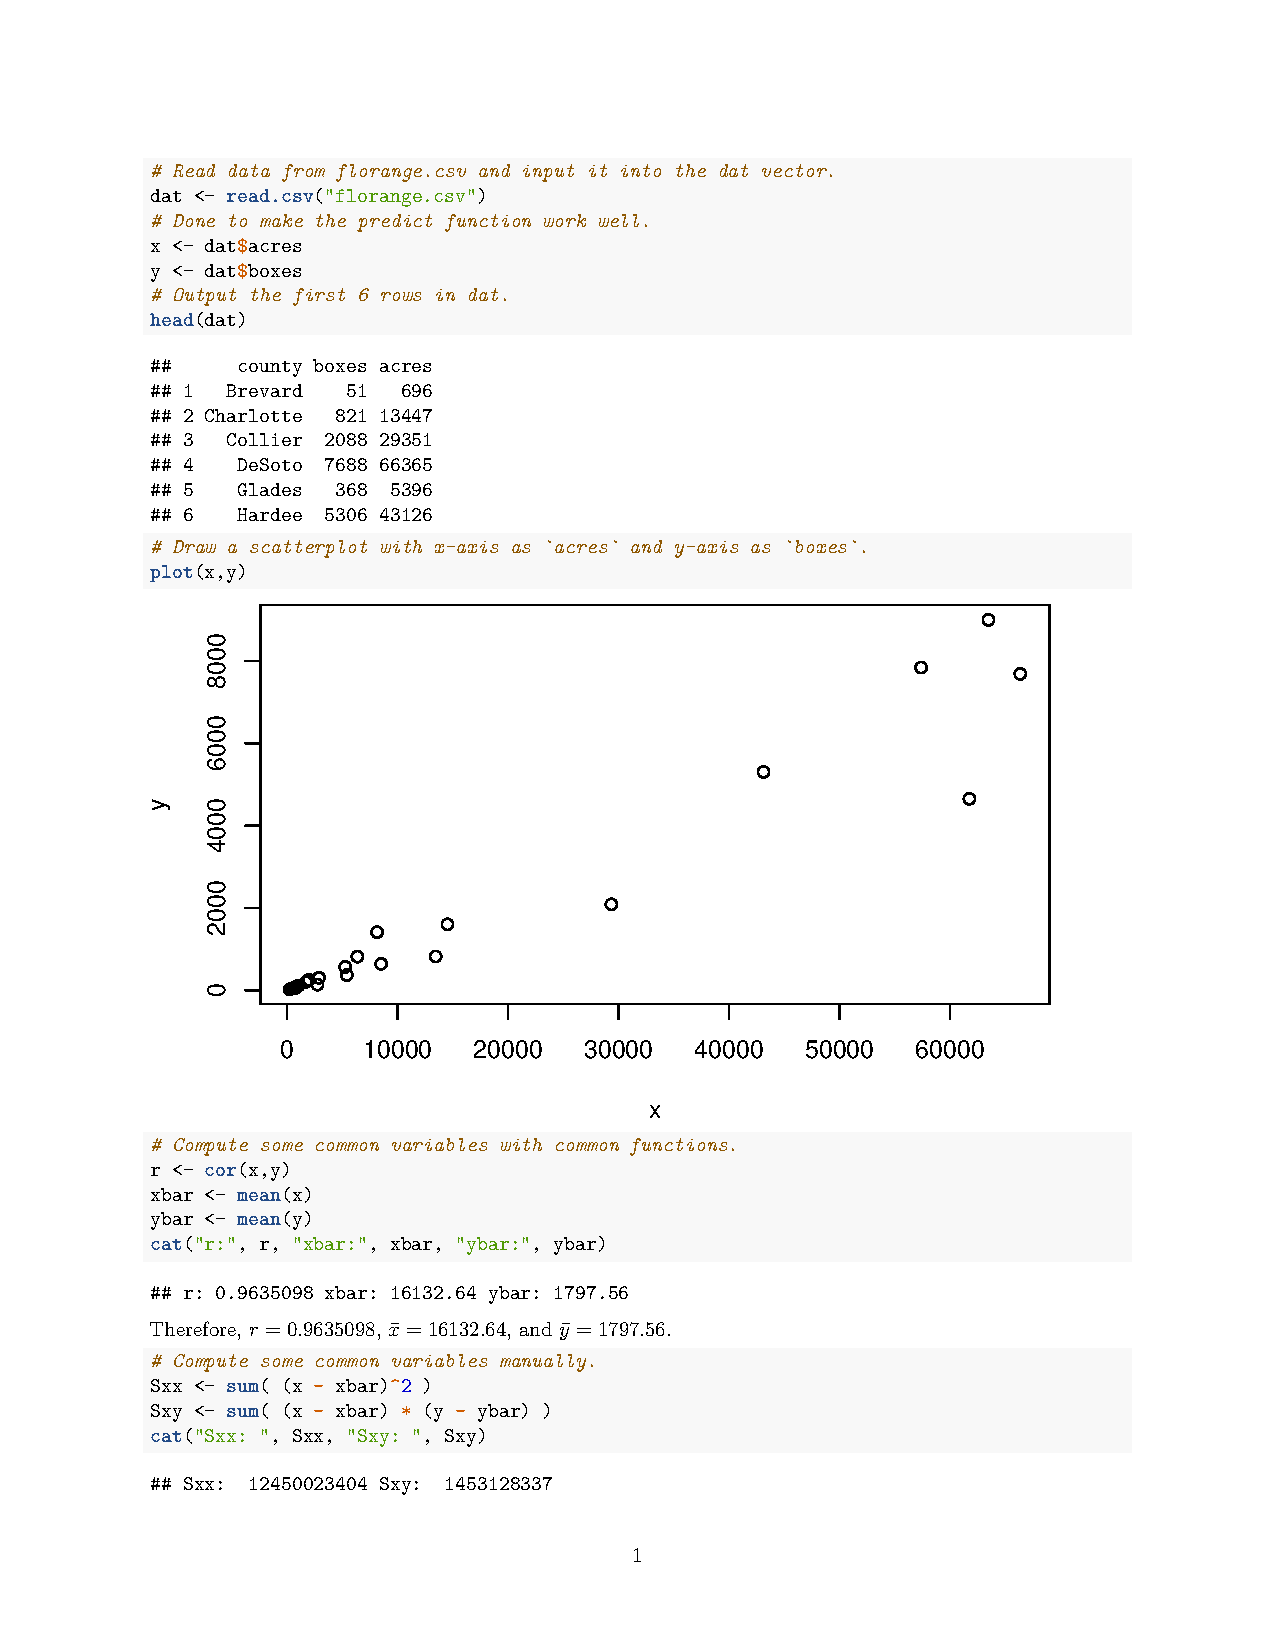
\includepdf[pages=-]{orange.pdf}
